%%%%%%%%%%%%%%%%%%%%%%%%%%%%%%%%%%%%%%%%%%%%%%%%%%%%%%%%%%%%%%%%%%%%%%
% Problem statement
\begin{statement}[
  problempoints=110,
  timelimit=10 seconds,
  memorylimit=512 MiB,
]{Skandi}

%\setlength\intextsep{-0.1cm}
%\begin{wrapfigure}[7]{r}{0.27\textwidth}
%\centering
%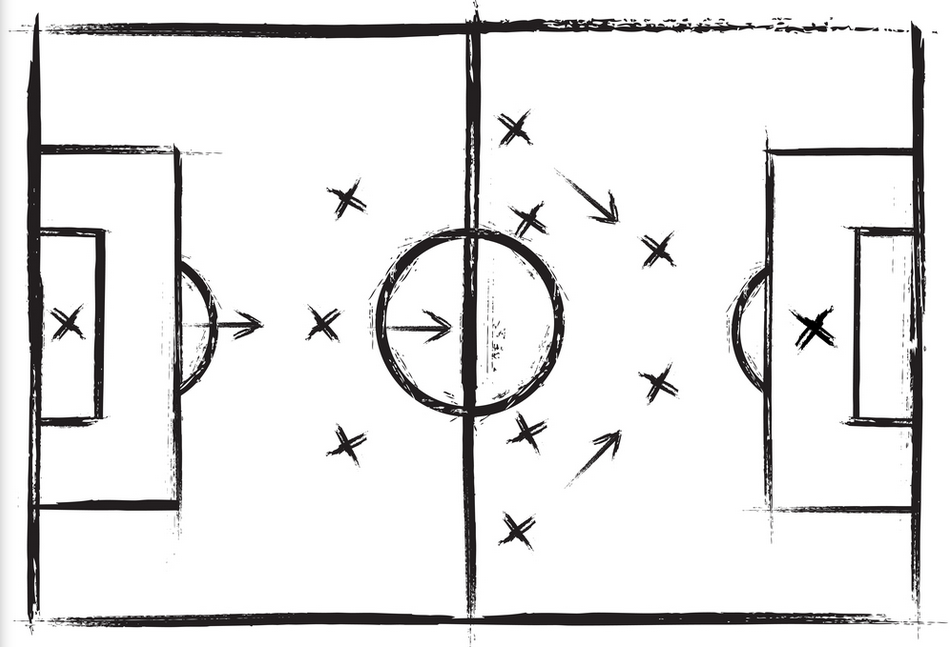
\includegraphics[width=0.27\textwidth]{img/trener.png}
%\end{wrapfigure}

Dragica is a captain of a local semi-professional bowling team, she is a
passionate chef and probably one of the best crossword puzzle solvers in
Croatia. A crossword puzzle consists of $N \times M$ squares arranged in $N$
rows and $M$ columns. Some of the squares are empty (and should be filled
with letters by answering questions) and some of the squares are filled.
Filled squares contain at most two questions which should either be answered
horizontally to the right or vertically downwards. The answers to the
questions are written in the empty squares before until we reach the
crossword bound or an initially-filled square.  An initially-filled square
contains a horizontal question if a square to the right exists and is empty.
Analogously, an initially-filled square contains a vertical question if a
square beneath it exists and is empty.

Dragica usually knows all the answers to the crossword puzzle questions, but
wishes to read and answer as little questions as possible and still solve the
entire crossword puzzle. Help her achieve her goal.

%%%%%%%%%%%%%%%%%%%%%%%%%%%%%%%%%%%%%%%%%%%%%%%%%%%%%%%%%%%%%%%%%%%%%%
% Input
\subsection*{Input}
The first line contains integers $N$ and $M$ $(2 \le N, M \le 500)$ from the
task description.

Each of the next $N$ lines contain $M$ characters \texttt{‘0’} or \texttt{‘1’},
where \texttt{‘0’} denotes an empty square which should be filled by
answering a question and \texttt{'1'} denotes an initially filled square
which may contain at most two questions as explained in the task description.
The first row and first column will be filled with \texttt{‘1’} characters.

It is guaranteed that there will be at least one character \texttt{'0'} in
the input.

%%%%%%%%%%%%%%%%%%%%%%%%%%%%%%%%%%%%%%%%%%%%%%%%%%%%%%%%%%%%%%%%%%%%%%
% Output
\subsection*{Output}
In the first line you should output the minimal number of questions that
can be answered in order to solve an entire crossword puzzle. Let's denote
that number with $X$.

Each of the next $X$ lines should describe one question that should be
answered.  The question description should be printed in the format \texttt{R
C direction}, where $R$ is the row number of the question, $C$ is the column
number of the question and direction is either \texttt{"DESNO"} (Croatian for
\texttt{RIGHT}) or \texttt{"DOLJE"} (Croatian for \texttt{DOWN}) depending on
whether Dragica should answer the vertical or horizontal question.

If there are multiple solutions, output any of them.

%%%%%%%%%%%%%%%%%%%%%%%%%%%%%%%%%%%%%%%%%%%%%%%%%%%%%%%%%%%%%%%%%%%%%%
% Scoring
\subsection*{Scoring}
{\renewcommand{\arraystretch}{1.4}
  \setlength{\tabcolsep}{6pt}
  \begin{tabular}{ccl}
 Subtask & Score & Constraints \\ \midrule
  1 & 18 & There will be at most $9$ squares with \texttt{'1'} \\
  2 & 32 & $N \le 500$ and $M \le 10$\\
  3 & 60 & No additional constraints. \\
\end{tabular}}

If your solution outputs the first line correctly on each test case of a
subtask, but it fails to correctly output the other lines in some test case,
you will score $50$\% of the allocated points for that subtask.

%%%%%%%%%%%%%%%%%%%%%%%%%%%%%%%%%%%%%%%%%%%%%%%%%%%%%%%%%%%%%%%%%%%%%%
% Examples
\subsection*{Examples}
\begin{tabularx}{\textwidth}{X'X'X}
\sampleinputs{test/skandi.dummy.in.1}{test/skandi.dummy.out.1} &
\sampleinputs{test/skandi.dummy.in.2}{test/skandi.dummy.out.2} &
\sampleinputs{test/skandi.dummy.in.3}{test/skandi.dummy.out.3}
\end{tabularx}

\textbf{Clarification of the third example:}
An example of a real crossword puzzle which is equivalent to the one described
in this example is given on the next page. Initially-filled squares are colored
black and those squares that contain at least one question are numerated. Below
the puzzle you can see the questions that should be solved \textit{to-the-right}
(column "across") and those that should be solved downwards (column "down").
Note that some initially-filled squares contain no questions, some contain
a single question (e.g. $8$ and $13$), while some contain two questions
(e.g. $10$ and $12$). In order to solve this crossword puzzle you need to
know the answers to at least $14$ questions that are listed in the output.
Can you solve it?

\setlength\intextsep{-0.5cm}
\begin{wrapfigure}{c}{\textwidth}
\centering
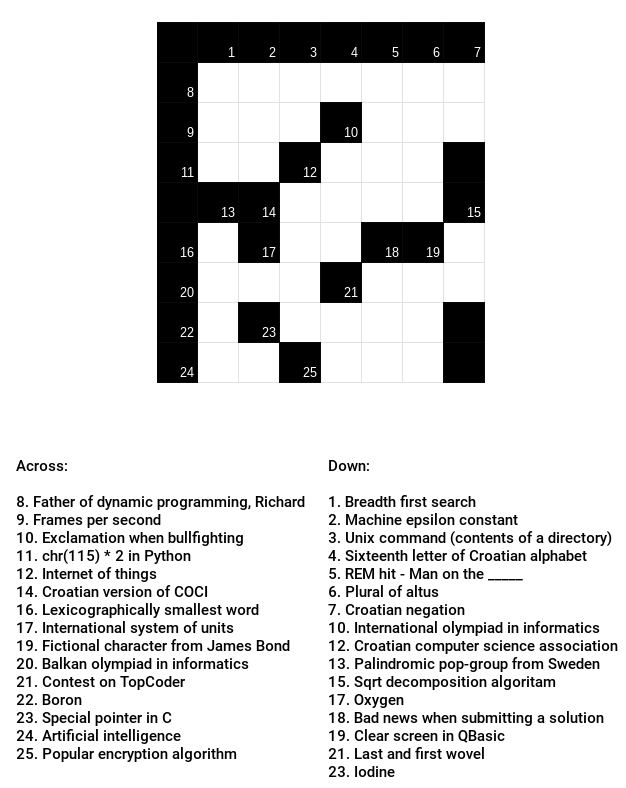
\includegraphics[width=0.8\textwidth]{skandi_en.png}
\end{wrapfigure}

%%%%%%%%%%%%%%%%%%%%%%%%%%%%%%%%%%%%%%%%%%%%%%%%%%%%%%%%%%%%%%%%%%%%%%
% We're done
\end{statement}

%%% Local Variables:
%%% mode: latex
%%% mode: flyspell
%%% ispell-local-dictionary: "croatian"
%%% TeX-master: "../hio.tex"
%%% End:
